\subsection{Choice of RX topology}

\IEEEPARstart{F}{or} the receiver we made several choices with regard to what topology and types of elements to use. The general topology we chose to use for the receiver is depicted in figure \ref{fig:topology}.

\begin{figure}[H]
  \centering
  {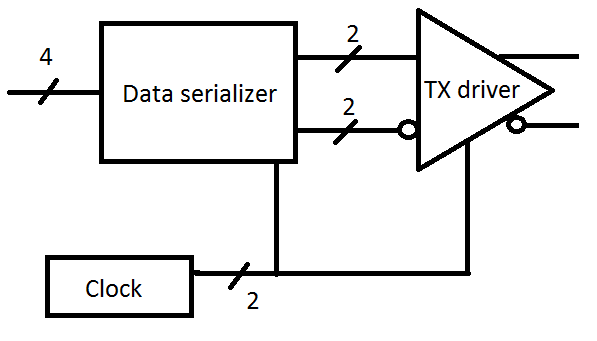
\includegraphics[scale=0.55]{img/topology_tx.png}}
  \caption{Transmitter top level topology}
  \label{fig:topology}
\end{figure}


The overall transceiver was to be a low-power 10 Gb/s link, and as such the receiver part of the link has to be power efficient like the transmitter. Thus we choose to base our topology on the design used in ~\cite{mahony2010a}, as this design implements a half-rate low-power link. As we chose to design our transmitter using half-rate clocking, it makes sense to implement a receiver with the same clock-rate, such that the clock can be forwarded to the receiver. We could have chosen not to forward the clock, but this would have generated the need to implement another clock-generator, which would add to the total power consumption.


Tuning of the termination impedance is done in the beginning of the receiver using several transistors and resistors in parallel, giving the possibility of tuning the impedance with a certain resolution.

The receiver is a 2-slice design as each slice is clocked at half-rate of the data, this introduces the need to implement a synchronizer after the slices but this can hopefully be implemented in low-power CMOS technology.

Each slice has a Track and Hold (sometimes called Sample and Hold) switch, depicted as "T/H" in figure \ref{fig:topology}.

For the buffer we chose to implement a VOA-3 differential amplifier as this should have a lower power penalty than a VOA-1 or VOA-2, and it is simpler to size than the VOA-4 amplifier. The VOA-3 differential amplifier utilizes a differential switched load in order to obtain a tunable offset, the tunable load is implemented through using several slices of transistors in the differential load.

For the strong-arm latch we chose to try and do our implementation with only one SAL instead of the two the use in ~\cite{mahony2010a}, in the hope of reducing the power consumption. If the load that the SAL needs to drive is too big to obtain the desired BW, we may need to introduce another SAL or re-think our receiver design.

We decided to not use CTLE nor DFE in the initial topology as these increase the power complexity of the receiver, we may need to add one or both of these later on if our signal needs more equalization.
